%
%----------------------------------------------------------------------------------------
%	PACKAGES AND DOCUMENT CONFIGURATIONS
%----------------------------------------------------------------------------------------
%

\documentclass[12pt]{article} %report, article, amsart, exam
\usepackage[letterpaper,margin=1in]{geometry}
\usepackage{fancyhdr,color}
\usepackage{tikz,graphicx,multicol}
\usepackage{amssymb,euscript,eufrak,nicefrac,enumitem}
\usepackage{amsfonts,amsmath,amsthm} %don't need with 'amsart' document class
\usepackage{hyperref}
\usepackage{comment}
\usepackage{scrextend} %needed for addmargin environment
\usepackage{graphicx} 
\usepackage{listings}

\usepackage{color}
\usepackage{accsupp}
\usepackage{booktabs}
\usepackage{subcaption}

\definecolor{dkblue}{rgb}{0,0,0.5}
\definecolor{comment}{rgb}{1,0,0}
\definecolor{mauve}{rgb}{.627,.126,.941}
\definecolor{purple}{rgb}{0.5, 0, 0.545098}

\lstdefinestyle{customc}{
  belowcaptionskip=1\baselineskip,
  breaklines=true,
  frame=L,
  xleftmargin=\parindent,
  language=C,
  showstringspaces=false,
  basicstyle=\footnotesize\ttfamily,
  keywordstyle=\bfseries\color{green!40!black},
  commentstyle=\itshape\color{purple!40!black},
  identifierstyle=\color{blue},
  stringstyle=\color{orange},
}

\lstdefinestyle{customasm}{
  belowcaptionskip=1\baselineskip,
  frame=L,
  xleftmargin=\parindent,
  language=[x86masm]Assembler,
  basicstyle=\footnotesize\ttfamily,
  commentstyle=\itshape\color{purple!40!black},
}

\lstset{escapechar=@,style=customc}

%
%----------------------------------------------------------------------------------------
%% Define headers & footers
%----------------------------------------------------------------------------------------

\pagestyle{fancy}
   \lhead{} 
   %\chead{Loyola University Chicago} 
   \rhead{}
   \renewcommand{\headrulewidth}{0pt}
   \addtolength{\footnotesep}{5mm}
 
%
%----------------------------------------------------------------------------------------
%% Some user-defined colors
%----------------------------------------------------------------

\setlength{\parskip}{1em}
\renewcommand{\baselinestretch}{1.3}

%
%----------------------------------------------------------------------------------------
%% BEGIN: HEADER
%----------------------------------------------------------------------------------------
%


\title{COMP 464 - High Performance Computing \\ High Frequency Trading Data Processing} % Title
\author{
Loyola University Chicago \\
Jose Luis Rodriguez 
} % Author name
\date{\today} % Date for the report

%
%------------------------------

\begin{document}

\maketitle

\thispagestyle{fancy}

%---------------------------------------------------------------------------------------- 
%	SECTION 1 - PROBLEM STATEMENT
%----------------------------------------------------------------------------------------

\section{Overview}

As computational capabilities continue to grow exponentially and financial markets around the world are increasingly dependent on automated systems, it is important to spend time analyzing market raw transactional data. Two approaches were developed - an openMP C++ application and a Spark/Hadoop application. Given the nature of the data (millions of transactions) it was necessary to implement the search, map, and reduce operations in parallel in order to efficiently process the market data. This report found that the openMP approach is easily scaleable and compatible with a multitude of hardware, despite its need for a more rigorous evaluation of code parallelization regions. 

The Spark/Hadoop approach can be seen as the go-to tool for large datasets (big data analysis) and was indeed easier to manipulate in so far as uploading data and conducting a preliminary analysis. With that said, the main drawback of the Spark/Hadoop approach is its lack of easy transferability. As soon as the Hadoop cluster is turned off, this approach is no longer functional. After the development, testing, and benchmark of the applications, the primary goal is to analyze the events leading up to the May 6, 2010 market flash crash. Preliminary findings on this project could be compared with the official report to congress from the CFTC and the SEC for additional work in the future. The data used in this project is from the CME Group and corresponds to market depth transactions in milliseconds of the E-Mini S\&P 500 futures and options contracts. 


%----------------------------------------------------------------
%	SECTION 2 - METHODOLOGY
%----------------------------------------------------------------

\section{Methodology}

%The ability to process a high volume of transactions and calculations in an ever-decreasing window of time has become a cornerstone of modern financial markets. With the advent of low-cost advanced computational capabilities and rapid growth market transactions, there must be a more accessible and efficient way to analyze raw financial data. Per the incidents highlighted in a joint report by the U.S. Securities \& Exchange Commission and The U.S. Commodity Futures Trading Commission, the months leading up to May of 2010 in the U.S were filled with political unrest overseas and news about the European debt crisis. On May 6, 2016, protections for the default of the Greek government's sovereign debt increased and the Euro declined sharply against the U.S Dollar and Japanese Yen. 

%This report highlights how volatile the afternoon of May 6, 2010 was in futures and securities markets. At some point the market was down 4\% from the previous day. The prices of futures contracts in particular stock index instruments declined suddenly another 5\%-6\% in a very short period of time before rebounding within a very short period of time. The complexities and more details of happened that day are covered in the mentioned report that was given to the senate Committee on Banking. Those details are beyond the scope of this project.

According to the CME Group Data Mine website, their market depth data provides all market data messages required to recreate the order book (list of orders that a trading firm uses to record the interest of buyers and sellers in a particular financial instrument). Each message contains between five to ten orders deep in futures markets and three orders deep in options markets. This data is timestamped to the millisecond, allowing for an in-depth analysis of the price and volume movement. 

To analyze the volume and price variation three main functions in openMP were utilized to first read the data into memory, search for a given tag that represents a value in the data, and finally (using the volume function) aggregate the results from the search method. These functions utilize openMP parallel pragmas in order to efficiently process the data. For benchmark purposes, different numbers of threads were used in order to identify the superior performance. For the Spark/Hadoop setup, the data reading process was different given the nature of the Hadoop. The data needed to be copied to the Hadoop cluster, then Spark was utilized for the analysis. While in Spark, a function to search for a given tag was created, and the results of the function were counted utilizing Spark parallelism features. 


%----------------------------------------------------------------
%	SECTION 3 - PERFORMANCE
%----------------------------------------------------------------

\section{Performance}

To measure performance, scalability metrics can be used in each of the map, search, reduce, and filtering operations. The performance measures are different depending upon the approach used. For openMP, it is possible to measure a number of performance metrics within the program, such as the time it takes to read a file into memory (RAM), the time it takes for a given number of threads to search a tag, and the time it takes to process and aggregate the results. In each of these functions, the time was recorded and a log was created. For the Spark/Hadoop approach, timing the operations was more direct as it is simply a matter of timing how long it takes to run a function. With that said, the Spark/Hadoop approach lacks the flexibility possessed by the openMP approach. A table and plots of the results of each approach can be found in the appendix. Further scaleability testing was possible utilizing the openMP approach as the number of threads can be increased to allow for quicker data processing.

\section{Conclusion}

The aim of this report was to highlight methods to approach high frequency trading data (raw market data) that can be utilized to conduct system and strategies backtesting and forensics of market transactions data. Addressing large transactional data sizes presents challenges in any setting, from transferring to opening, and even regarding storage resources. In many cases, raw financial transactional data is not stored in a common data type. Special search functions must be implemented in order to parse the data and make the data usable. Finally, having access to raw transaction data is proven to be a very challenging task, as these datasets are very costly and the amount of time and resources that these datasets demand can be prohibitive for companies and/or researchers. Nonetheless, it is in the best interest of all that applications such as the one built in this project are created and are open source. There is an opportunity to create a robust community that could lead the charge on increasing transparency, education, and training in the high frequency trading industry.


%----------------------------------------------------------------
%	SECTION 4 - REFERENCE
%----------------------------------------------------------------

\newpage

\section{Reference}

\begin{flushleft}

TACC Wrangler User Guide  -- The Wrangler Data Analysis and Storage System \url{https://portal.tacc.utexas.edu/user-guides/wrangler}

Stampede2 User Guide -- Supercomputer at the Texas Advanced Computing Center \url{https://portal.tacc.utexas.edu/user-guides/stampede2}

Introduction to High Performance Scientific Computing -- Victor Eijkhout \\ \url{http://pages.tacc.utexas.edu/~eijkhout/istc/istc.html}

Kirilenko, Andrei; Kyle, Albert S.; Samadi, Mehrdad; Tuzun, Tugkan (May 5, 2014), The Flash Crash: The Impact of High Frequency Trading on an Electronic Market (PDF), retrieved 8 November 2017 \\ \url{http://www.cftc.gov/idc/groups/public/@economicanalysis/documents/file/oce_flashcrash0314.pdf}

Findings Regarding the Market Events of May 6, 2010 (Rep.). (2010, September 20). Retrieved December 12, 2017, from U.S. Securities \& Exchange Commission website: https://www.sec.gov/news/studies/2010/marketevents-report.pdf

\end{flushleft}

\newpage

\section{Appendix}

\begin{figure}[htb]
\caption{Read [50,846,717] - 05/02/10 - 05/08/10 - Speed-Up (T1/Tp)}\label{fig:benchmark01}
\centering
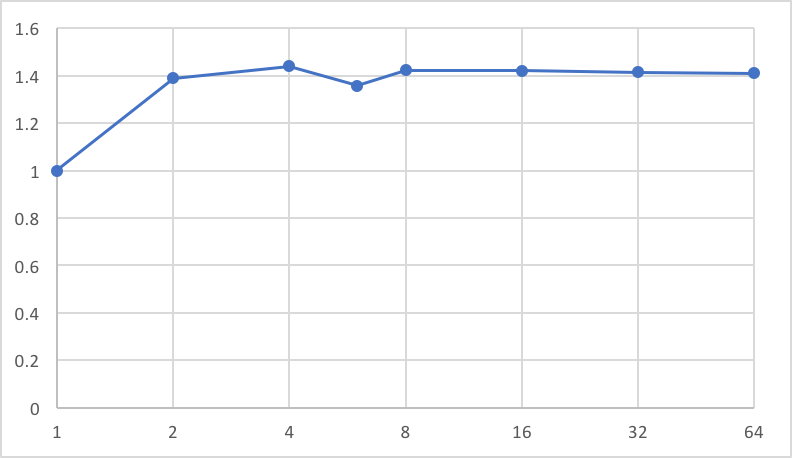
\includegraphics[width=15cm,keepaspectratio]{imgs/img01.png}
\end{figure} 

\begin{figure}[htb]
\caption{Read [50,846,717] - 05/02/10 - 05/08/10 - Efficiency (T1/Tp)}\label{fig:benchmark01}
\centering
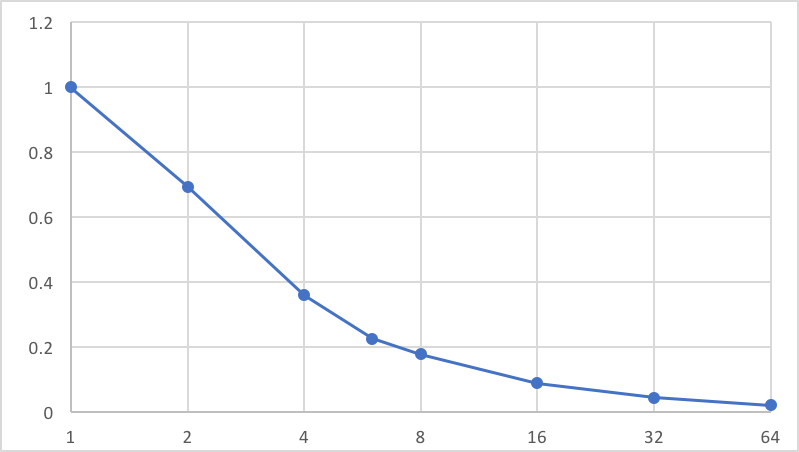
\includegraphics[width=15cm,keepaspectratio]{imgs/img02.png}
\end{figure} 

\begin{figure}[htb]
\caption{Search [50,846,717] - 05/02/10 - 05/08/10 - Speed-Up (T1/Tp)}\label{fig:benchmark01}
\centering
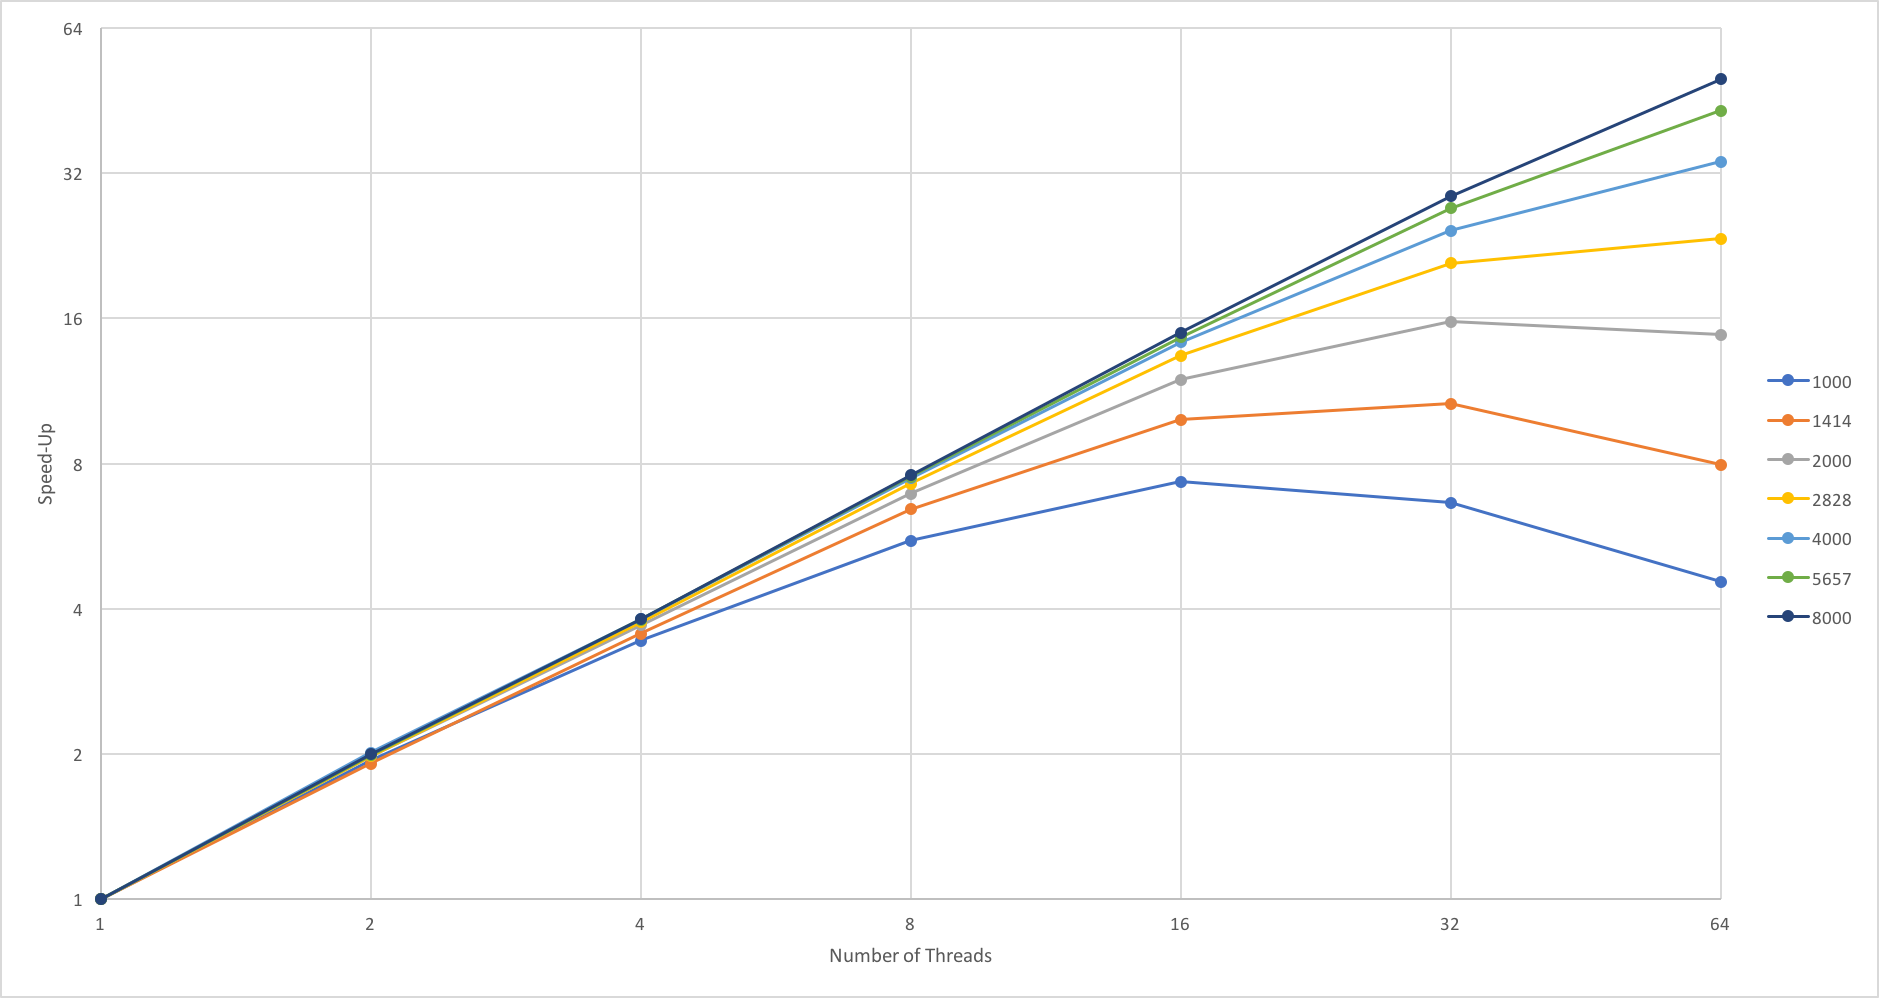
\includegraphics[width=15cm,keepaspectratio]{imgs/img03.png}
\end{figure} 

\begin{figure}[htb]
\caption{Search [50,846,717] - 05/02/10 - 05/08/10 - Efficiency (T1/Tp)}\label{fig:benchmark01}
\centering
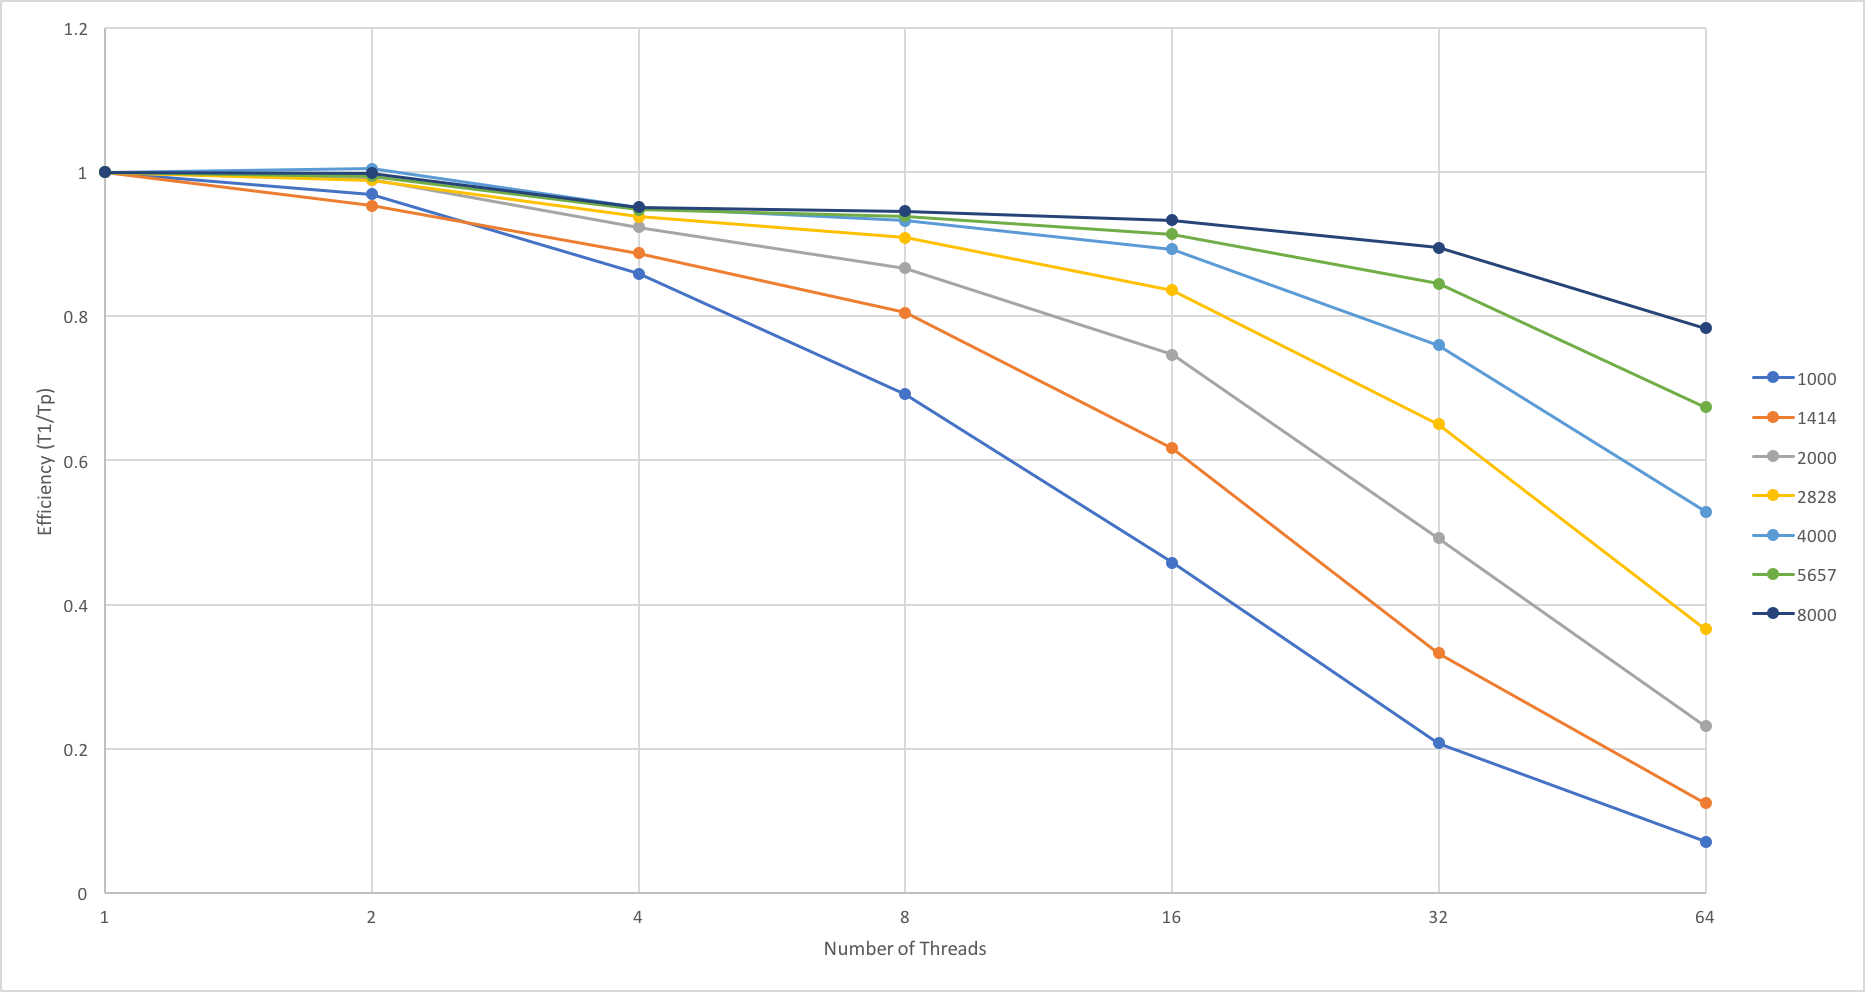
\includegraphics[width=15cm,keepaspectratio]{imgs/img04.png}
\end{figure} 

\begin{figure}[htb]
\caption{Volume [50,846,717] - 05/02/10 - 05/08/10 - Speed-Up (T1/Tp)}\label{fig:benchmark01}
\centering
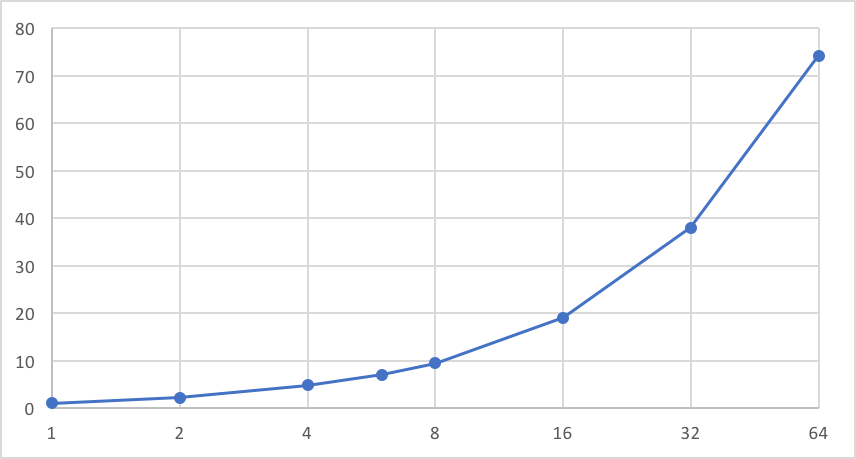
\includegraphics[width=15cm,keepaspectratio]{imgs/img05.png}
\end{figure} 

\begin{figure}[htb]
\caption{Volume [50,846,717] - 05/02/10 - 05/08/10 - Efficiency (T1/Tp)}\label{fig:benchmark01}
\centering
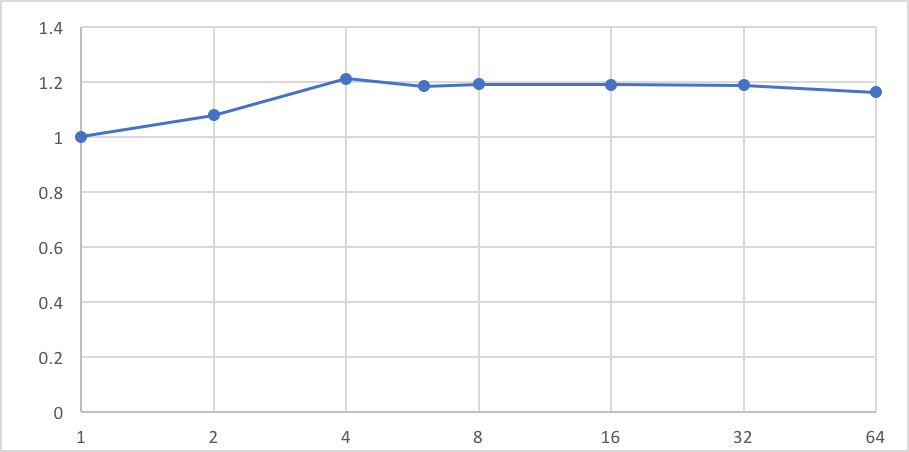
\includegraphics[width=15cm,keepaspectratio]{imgs/img06.png}
\end{figure} 

% Read Speed-up-[43,593,190] - 05/09/10 - 05/15/10

\begin{figure}[htb]
\caption{Read [43,593,190] - 05/09/10 - 05/15/10 - Speed-Up (T1/Tp)}\label{fig:benchmark01}
\centering
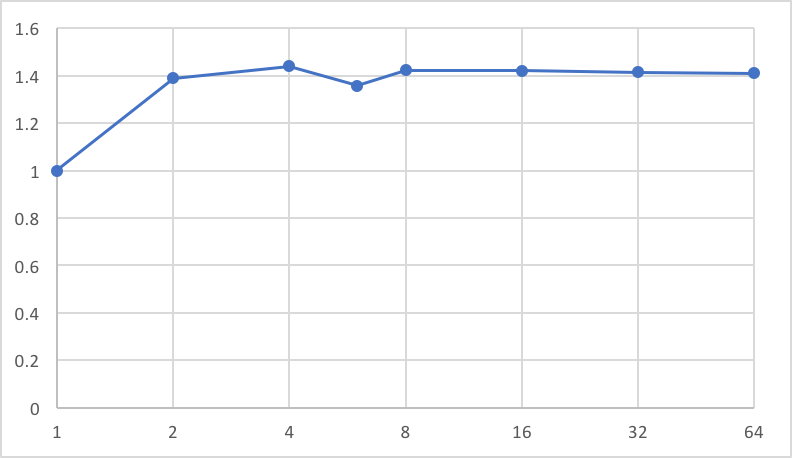
\includegraphics[width=15cm,keepaspectratio]{imgs/img01.png}
\end{figure} 

\begin{figure}[htb]
\caption{Read [43,593,190] - 05/09/10 - 05/15/10 - Efficiency (T1/Tp)}\label{fig:benchmark01}
\centering
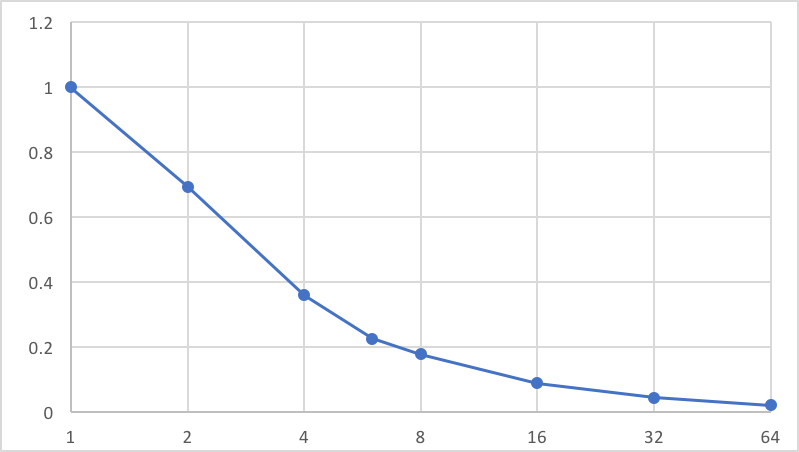
\includegraphics[width=15cm,keepaspectratio]{imgs/img02.png}
\end{figure} 

\begin{figure}[htb]
\caption{Search [43,593,190] - 05/09/10 - 05/15/10 - Speed-Up (T1/Tp)}\label{fig:benchmark01}
\centering
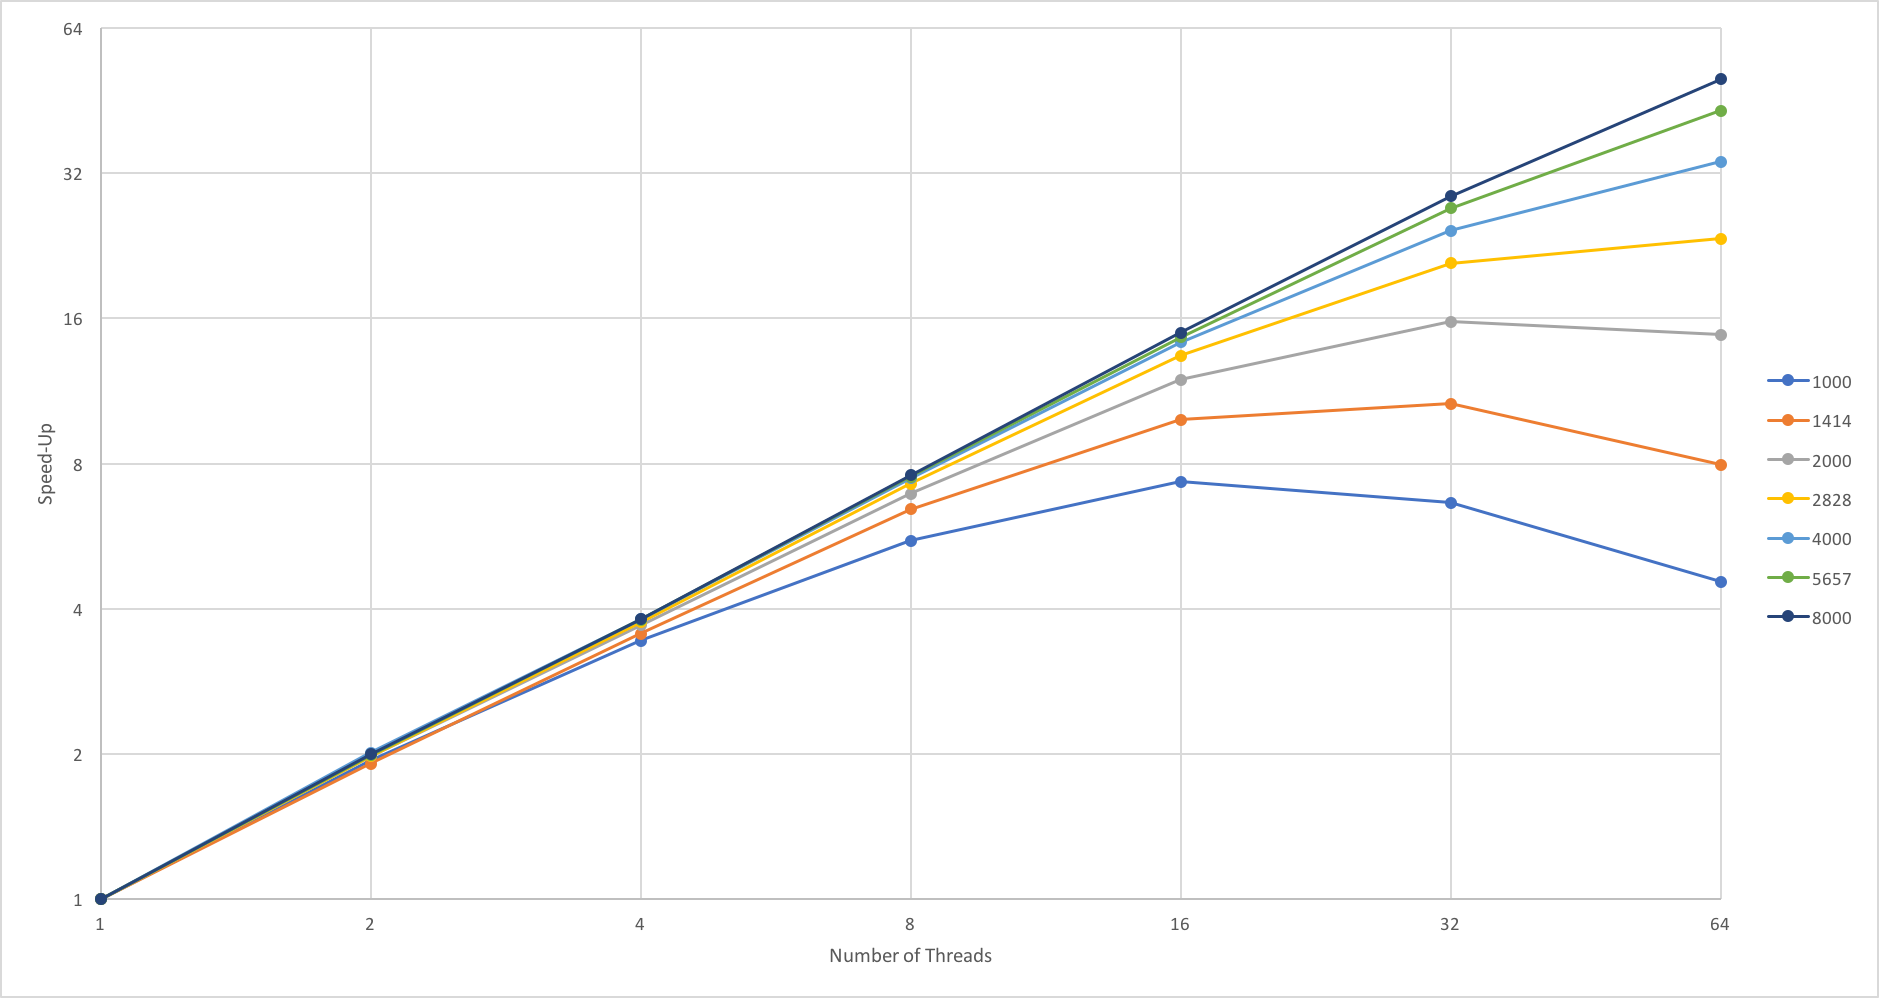
\includegraphics[width=15cm,keepaspectratio]{imgs/img03.png}
\end{figure} 

\begin{figure}[htb]
\caption{Search [43,593,190] - 05/09/10 - 05/15/10 - Efficiency (T1/Tp)}\label{fig:benchmark01}
\centering
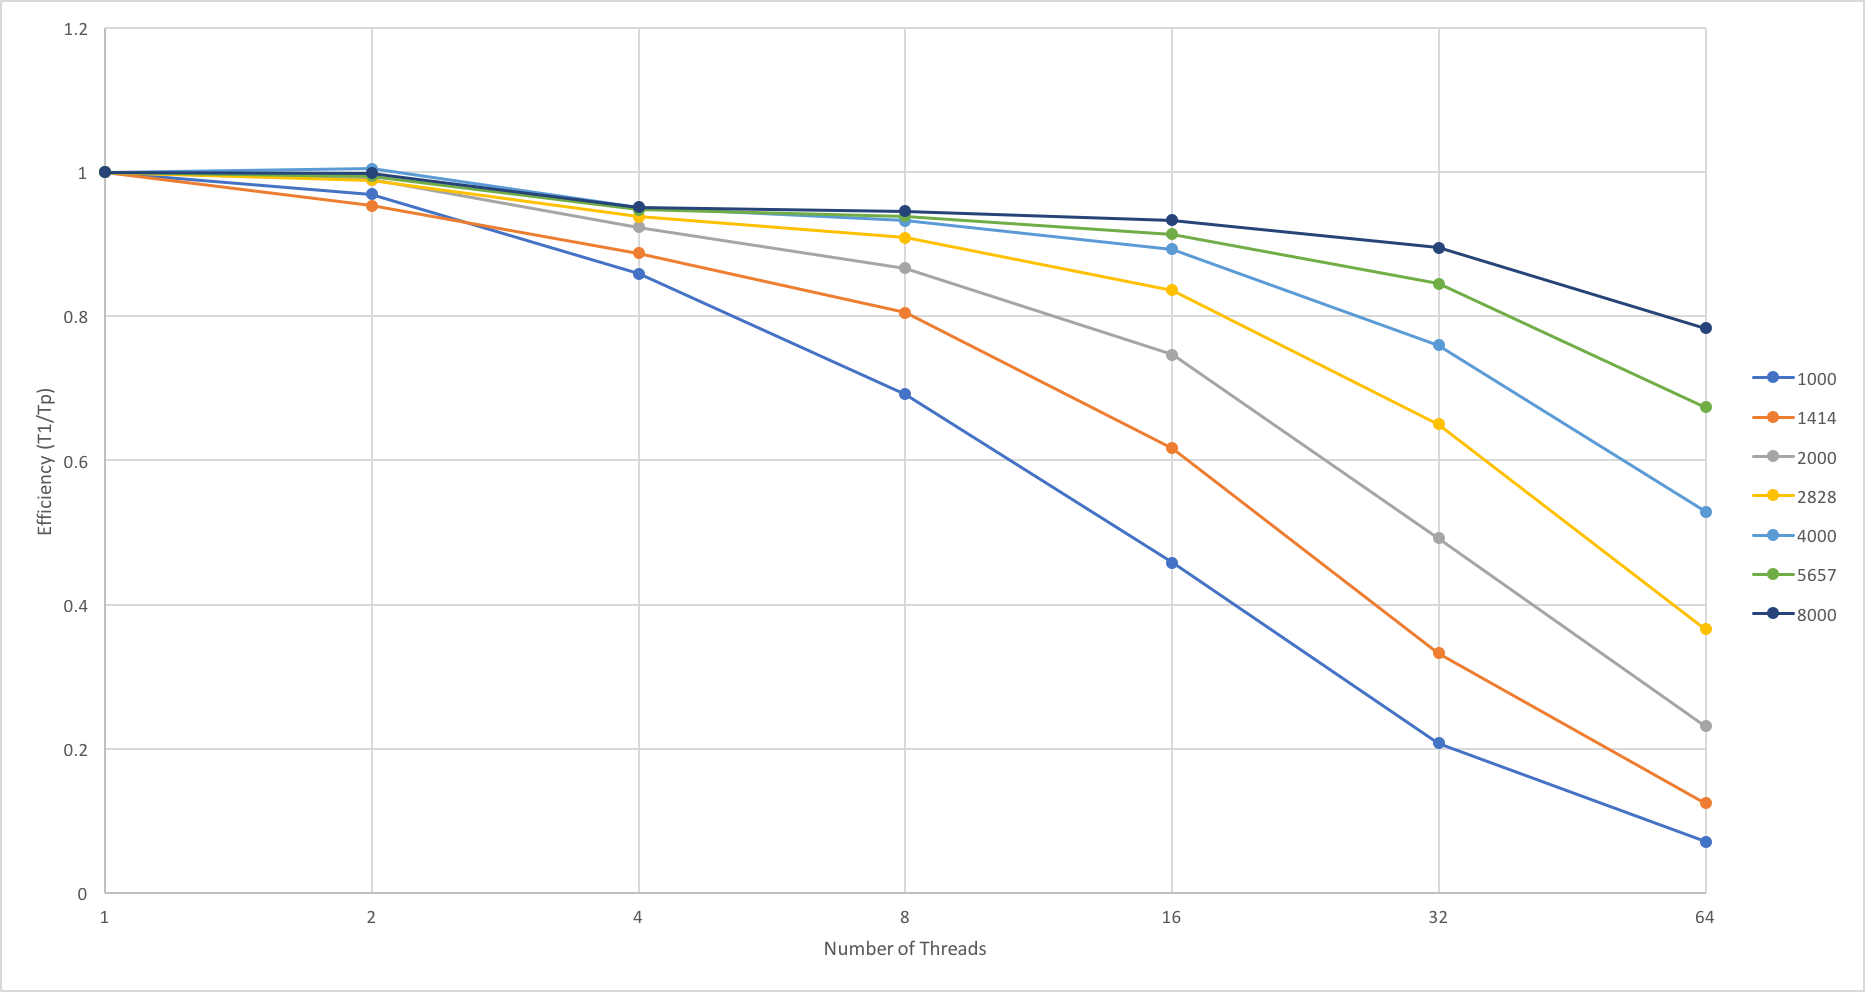
\includegraphics[width=15cm,keepaspectratio]{imgs/img04.png}
\end{figure} 

\begin{figure}[htb]
\caption{Volume [43,593,190] - 05/09/10 - 05/15/10 - Speed-Up (T1/Tp)}\label{fig:benchmark01}
\centering
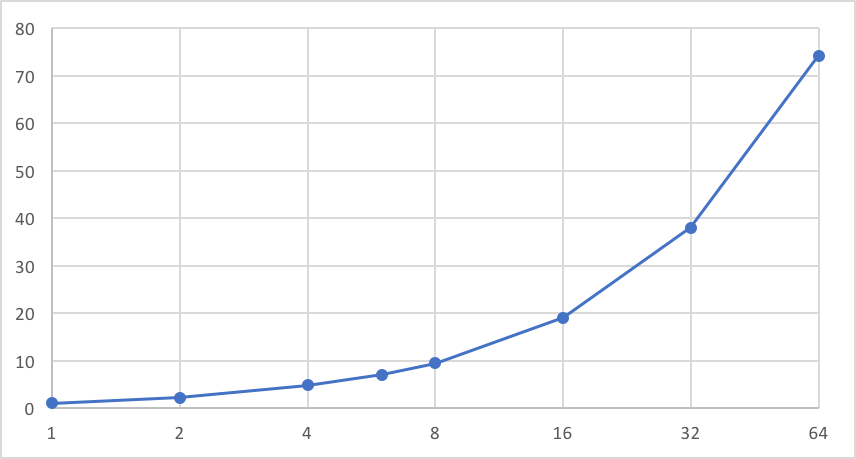
\includegraphics[width=15cm,keepaspectratio]{imgs/img05.png}
\end{figure} 

\begin{figure}[htb]
\caption{Volume [43,593,190] - 05/09/10 - 05/15/10 - Efficiency (T1/Tp)}\label{fig:benchmark01}
\centering
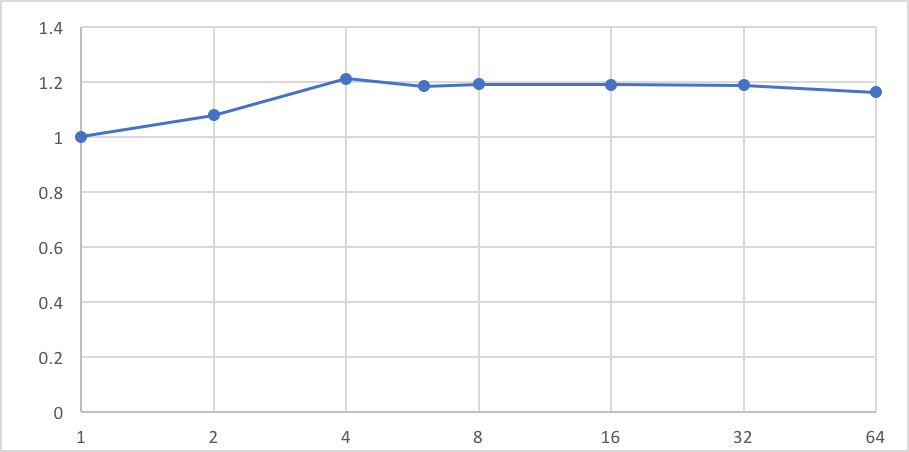
\includegraphics[width=15cm,keepaspectratio]{imgs/img06.png}
\end{figure} 

%Read Speed-up-[62,586,111]- 05/16/10 - 05/22/10

\begin{figure}[htb]
\caption{Read [62,586,111]- 05/16/10 - 05/22/10 - Speed-Up (T1/Tp)}\label{fig:benchmark01}
\centering
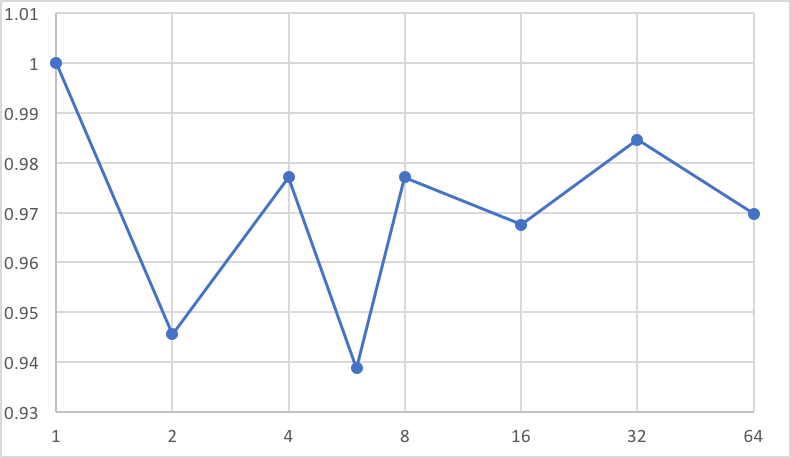
\includegraphics[width=15cm,keepaspectratio]{imgs/img07.png}
\end{figure} 

\begin{figure}[htb]
\caption{Read [62,586,111]- 05/16/10 - 05/22/10 - Efficiency (T1/Tp)}\label{fig:benchmark01}
\centering
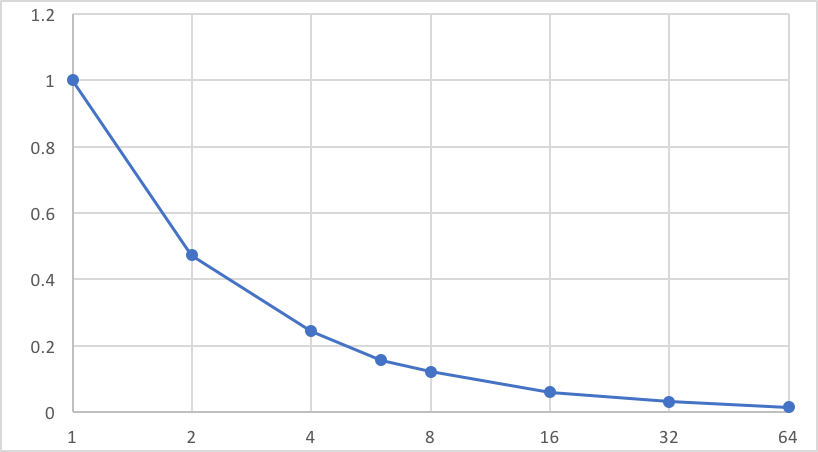
\includegraphics[width=15cm,keepaspectratio]{imgs/img08.png}
\end{figure} 

\begin{figure}[htb]
\caption{Search [62,586,111]- 05/16/10 - 05/22/10 - Speed-Up (T1/Tp)}\label{fig:benchmark01}
\centering
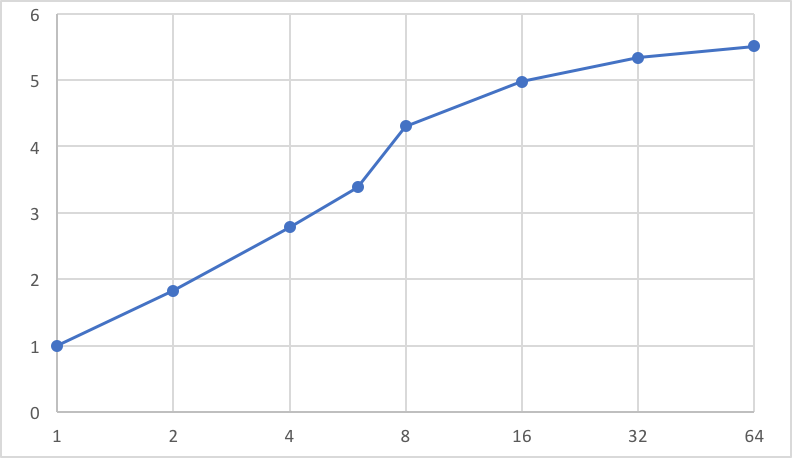
\includegraphics[width=15cm,keepaspectratio]{imgs/img09.png}
\end{figure} 

\begin{figure}[htb]
\caption{Search [62,586,111]- 05/16/10 - 05/22/10 - Efficiency (T1/Tp)}\label{fig:benchmark01}
\centering
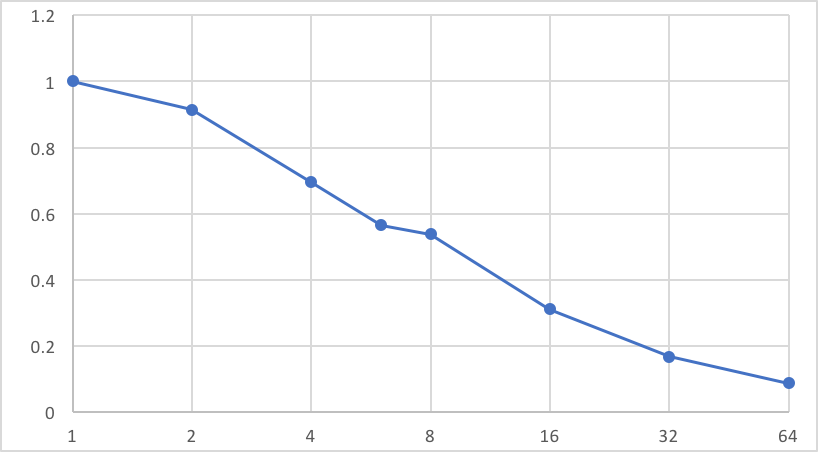
\includegraphics[width=15cm,keepaspectratio]{imgs/img10.png}
\end{figure} 

\begin{figure}[htb]
\caption{Volume [62,586,111]- 05/16/10 - 05/22/10 - Speed-Up (T1/Tp)}\label{fig:benchmark01}
\centering
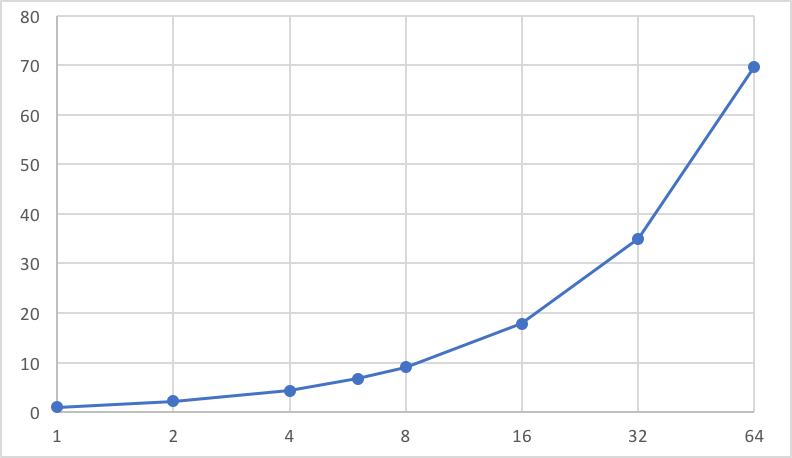
\includegraphics[width=15cm,keepaspectratio]{imgs/img11.png}
\end{figure} 

\begin{figure}[htb]
\caption{Volume [62,586,111]- 05/16/10 - 05/22/10 - Efficiency (T1/Tp)}\label{fig:benchmark01}
\centering
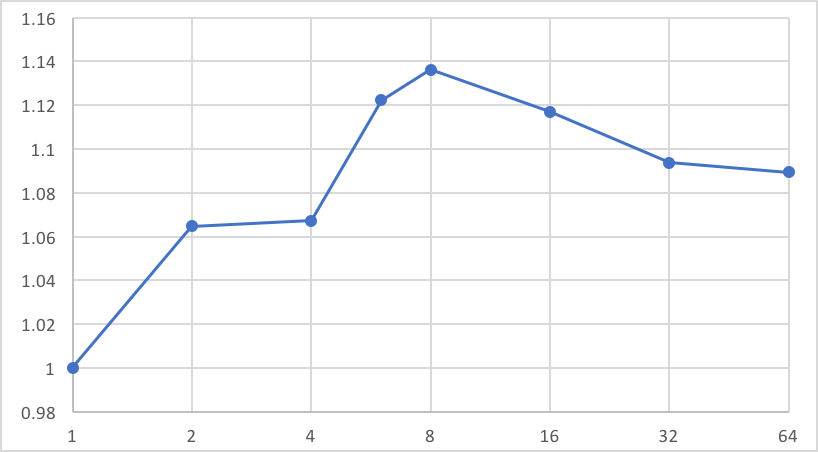
\includegraphics[width=15cm,keepaspectratio]{imgs/img12.png}
\end{figure} 

%Read Speed-up-[41,407,982]- 05/23/10 - 05/30/10

\begin{figure}[htb]
\caption{Read [41,407,982]- 05/23/10 - 05/30/10 - Speed-Up (T1/Tp)}\label{fig:benchmark01}
\centering
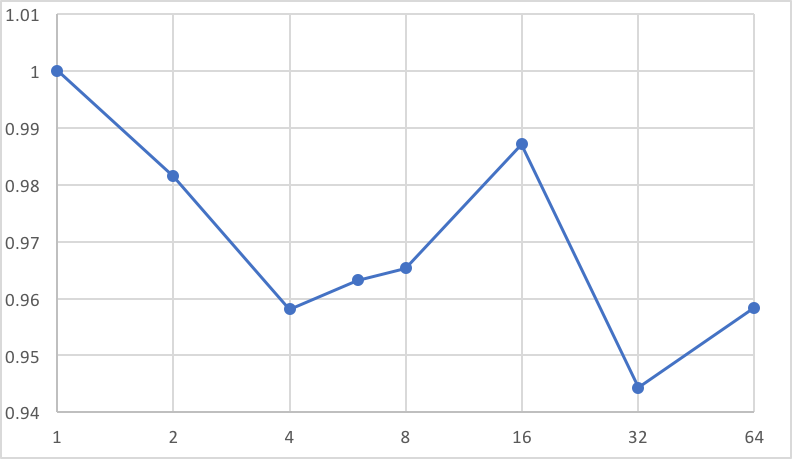
\includegraphics[width=15cm,keepaspectratio]{imgs/img13.png}
\end{figure} 

\begin{figure}[htb]
\caption{Read [41,407,982]- 05/23/10 - 05/30/10 - Efficiency (T1/Tp)}\label{fig:benchmark01}
\centering
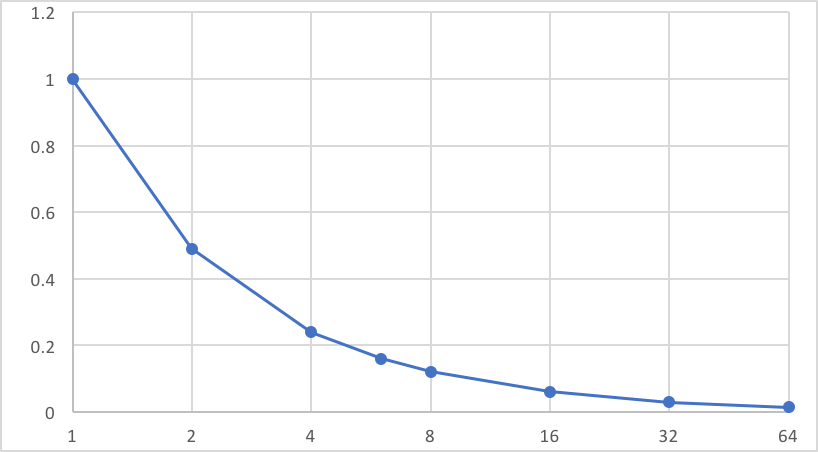
\includegraphics[width=15cm,keepaspectratio]{imgs/img14.png}
\end{figure} 

\begin{figure}[htb]
\caption{Search [41,407,982]- 05/16/10 - 05/22/10 - Speed-Up (T1/Tp)}\label{fig:benchmark01}
\centering
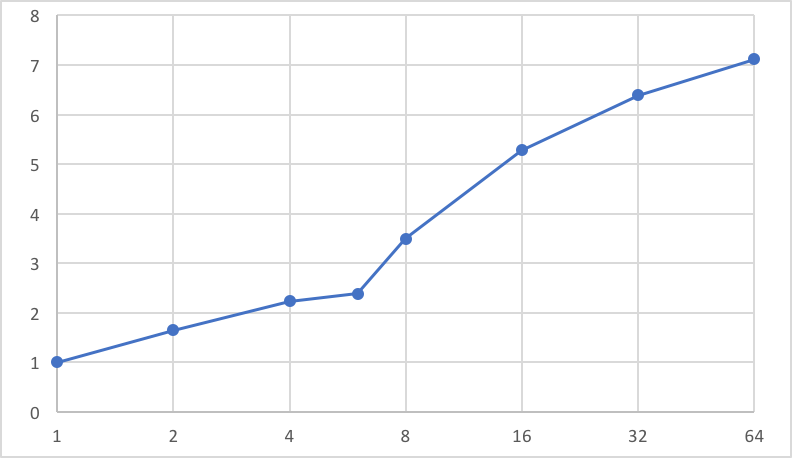
\includegraphics[width=15cm,keepaspectratio]{imgs/img15.png}
\end{figure} 

\begin{figure}[htb]
\caption{Search [41,407,982]- 05/16/10 - 05/22/10 - Efficiency (T1/Tp)}\label{fig:benchmark01}
\centering
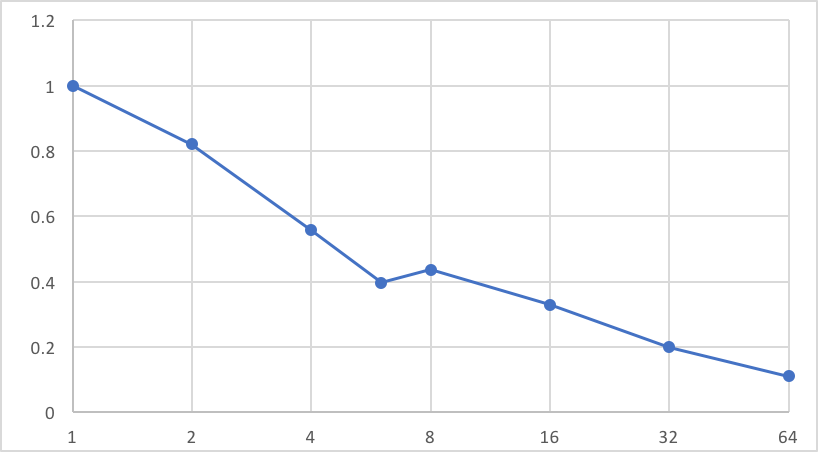
\includegraphics[width=15cm,keepaspectratio]{imgs/img16.png}
\end{figure} 

\begin{figure}[htb]
\caption{Volume [41,407,982]- 05/16/10 - 05/22/10 - Speed-Up (T1/Tp)}\label{fig:benchmark01}
\centering
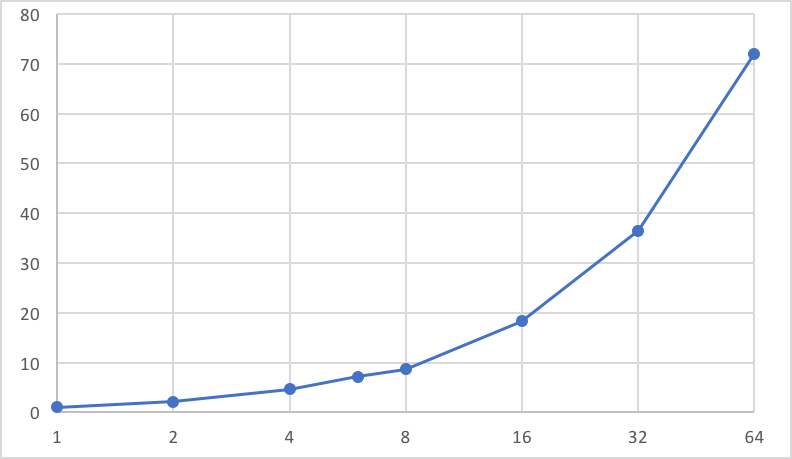
\includegraphics[width=15cm,keepaspectratio]{imgs/img17.png}
\end{figure} 

\begin{figure}[htb]
\caption{Volume [41,407,982]- 05/16/10 - 05/22/10 - Efficiency (T1/Tp)}\label{fig:benchmark01}
\centering
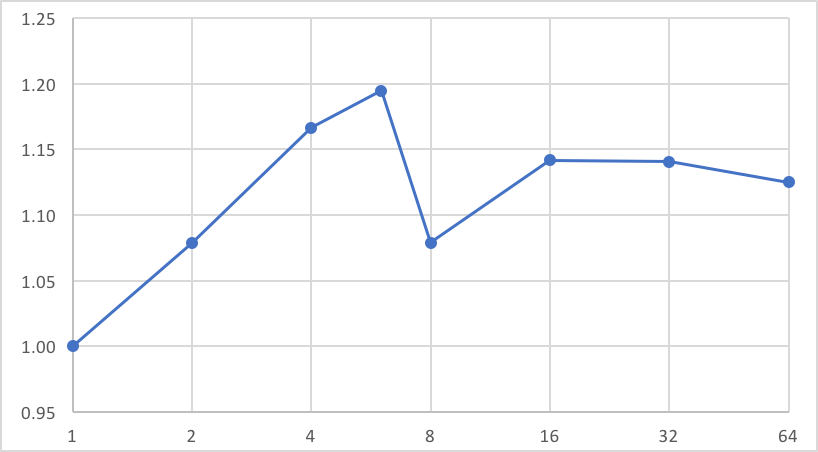
\includegraphics[width=15cm,keepaspectratio]{imgs/img18.png}
\end{figure} 


%Read Speed-up-[31,720,486]- 05/30/10 - 06/03/10

\begin{figure}[htb]
\caption{Read [31,720,486]- 05/30/10 - 06/03/10 - Speed-Up (T1/Tp)}\label{fig:benchmark01}
\centering
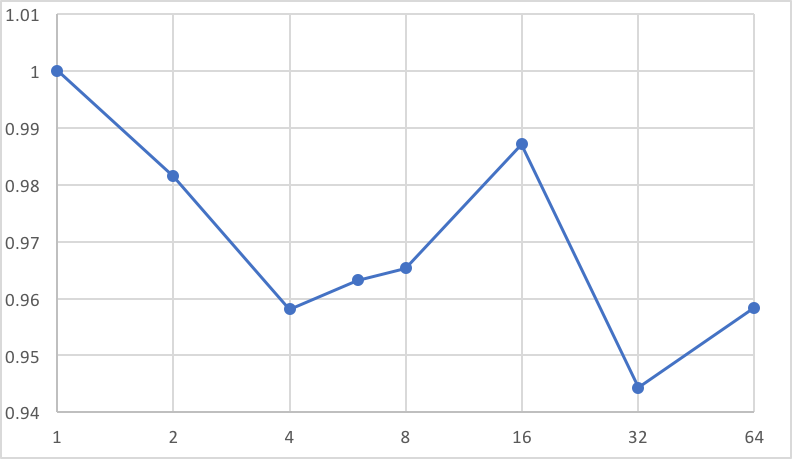
\includegraphics[width=15cm,keepaspectratio]{imgs/img13.png}
\end{figure} 

\begin{figure}[htb]
\caption{Read [31,720,486]- 05/30/10 - 06/03/10 - Efficiency (T1/Tp)}\label{fig:benchmark01}
\centering
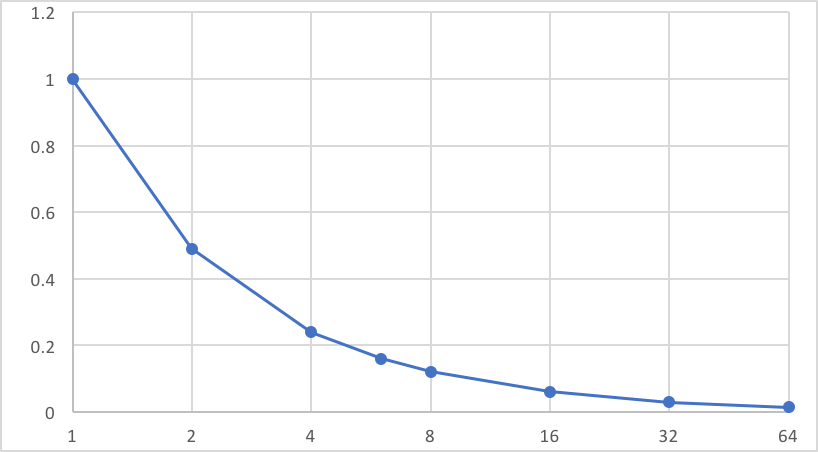
\includegraphics[width=15cm,keepaspectratio]{imgs/img14.png}
\end{figure} 

\begin{figure}[htb]
\caption{Search [31,720,486]- 05/30/10 - 06/03/10 - Speed-Up (T1/Tp)}\label{fig:benchmark01}
\centering
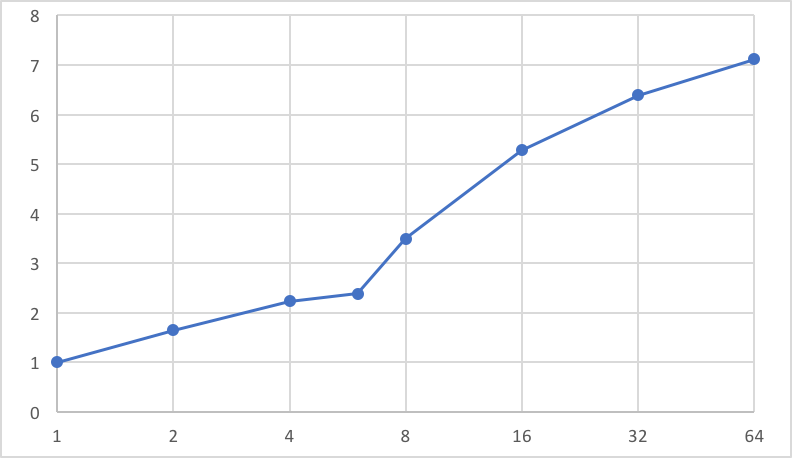
\includegraphics[width=15cm,keepaspectratio]{imgs/img15.png}
\end{figure} 

\begin{figure}[htb]
\caption{Search [31,720,486]- 05/30/10 - 06/03/10 - Efficiency (T1/Tp)}\label{fig:benchmark01}
\centering
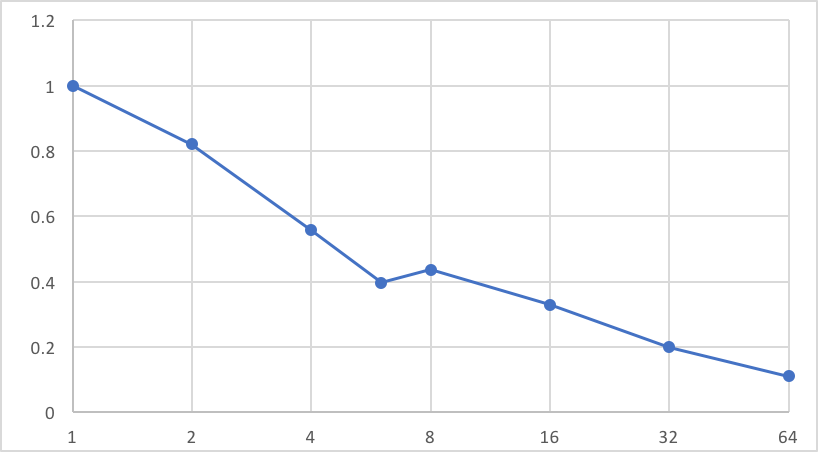
\includegraphics[width=15cm,keepaspectratio]{imgs/img16.png}
\end{figure} 

\begin{figure}[htb]
\caption{Volume [31,720,486]- 05/30/10 - 06/03/10 - Speed-Up (T1/Tp)}\label{fig:benchmark01}
\centering
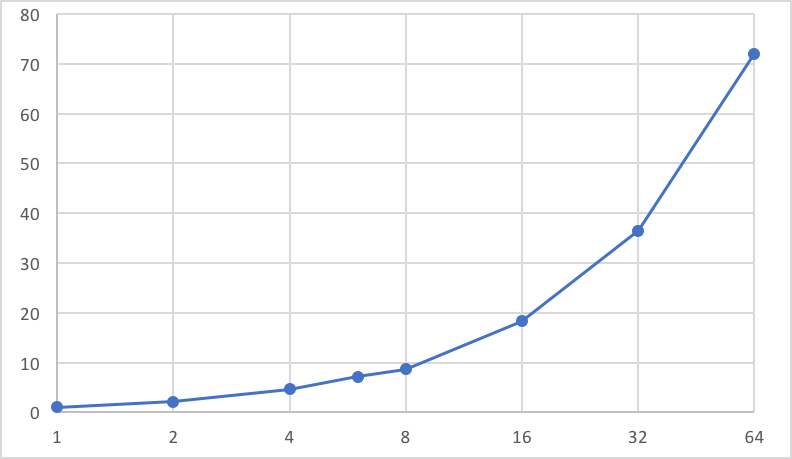
\includegraphics[width=15cm,keepaspectratio]{imgs/img17.png}
\end{figure} 

\begin{figure}[htb]
\caption{Volume [31,720,486]- 05/30/10 - 06/03/10 - Efficiency (T1/Tp)}\label{fig:benchmark01}
\centering
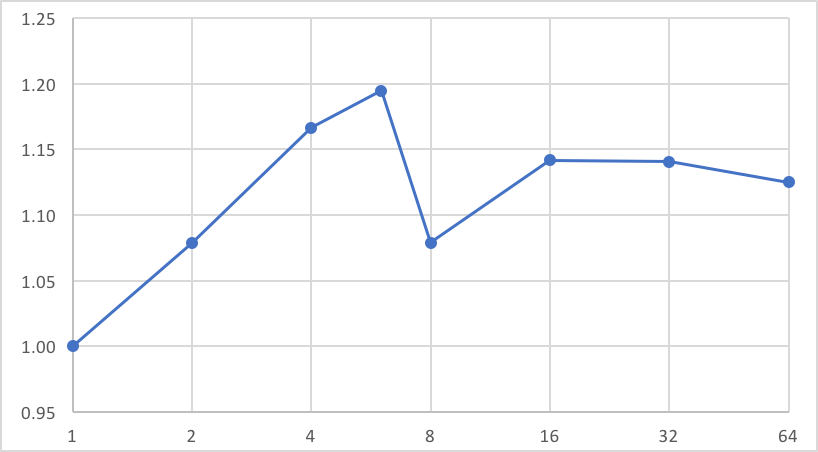
\includegraphics[width=15cm,keepaspectratio]{imgs/img18.png}
\end{figure} 


\end{document}